\documentclass[12pt]{article} 
\usepackage{graphicx}
\usepackage{float}
\graphicspath{ {./} }
\begin{document}
	%%%%%%%%%%%%% default mark-up %%%%%%%%%%%%%
	\title{Laboratory Assessment 2: Parallel Computing}
	\author{Student 1076589}
	\maketitle
	\pagebreak
	
	\section{Vector dot product:}
	
	\textbf{1.1)} Parallelization is useful in the problem of the dot product as it contains indepenedt operations (ai*bi) that are repeated over the vector. In this case, we parallelize the multiplication of the vlaue pairs in the vectors, each thread adding independantly, and summing the partial sums. \newline
	\begin{figure}[H]
		\centering
		\begin{center}
			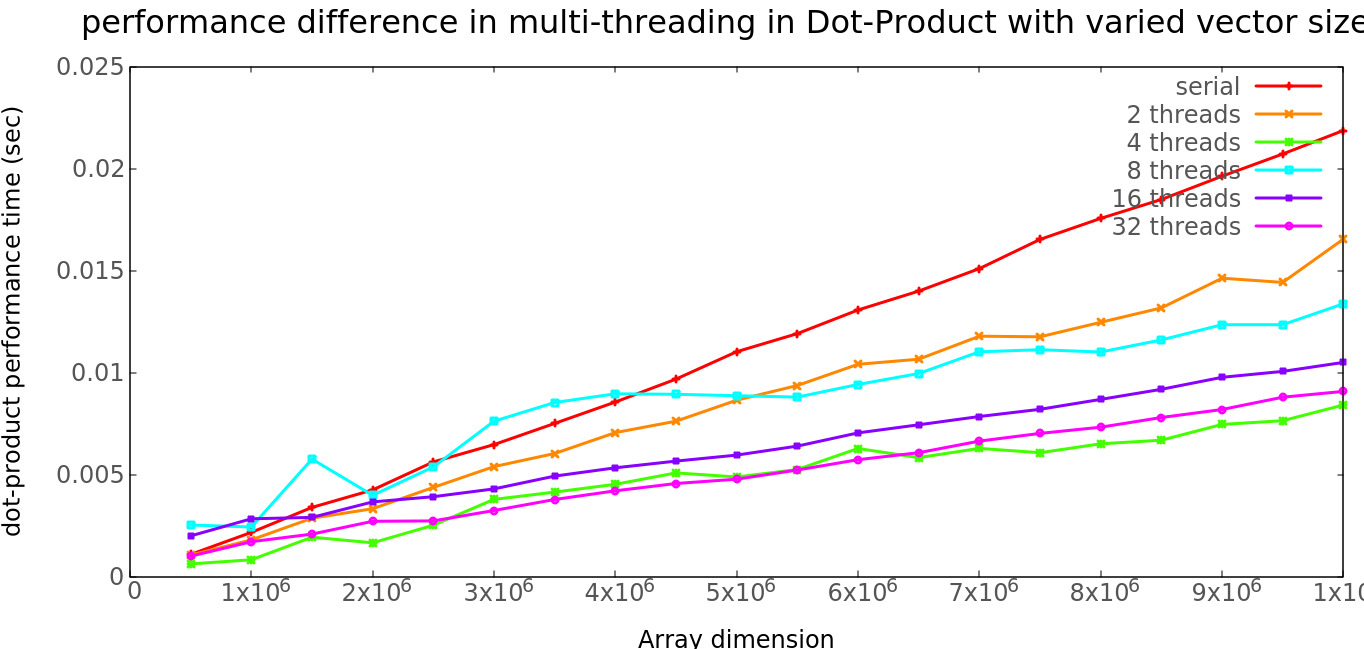
\includegraphics[width=1.00\textwidth]{graph1.png}
		\end{center}		
		\caption{Line plot of array dimension vs operation time, comparing serial and threaded dot-product}
	\end{figure}
	\begin{figure}[H]
		\centering
		\begin{center}
			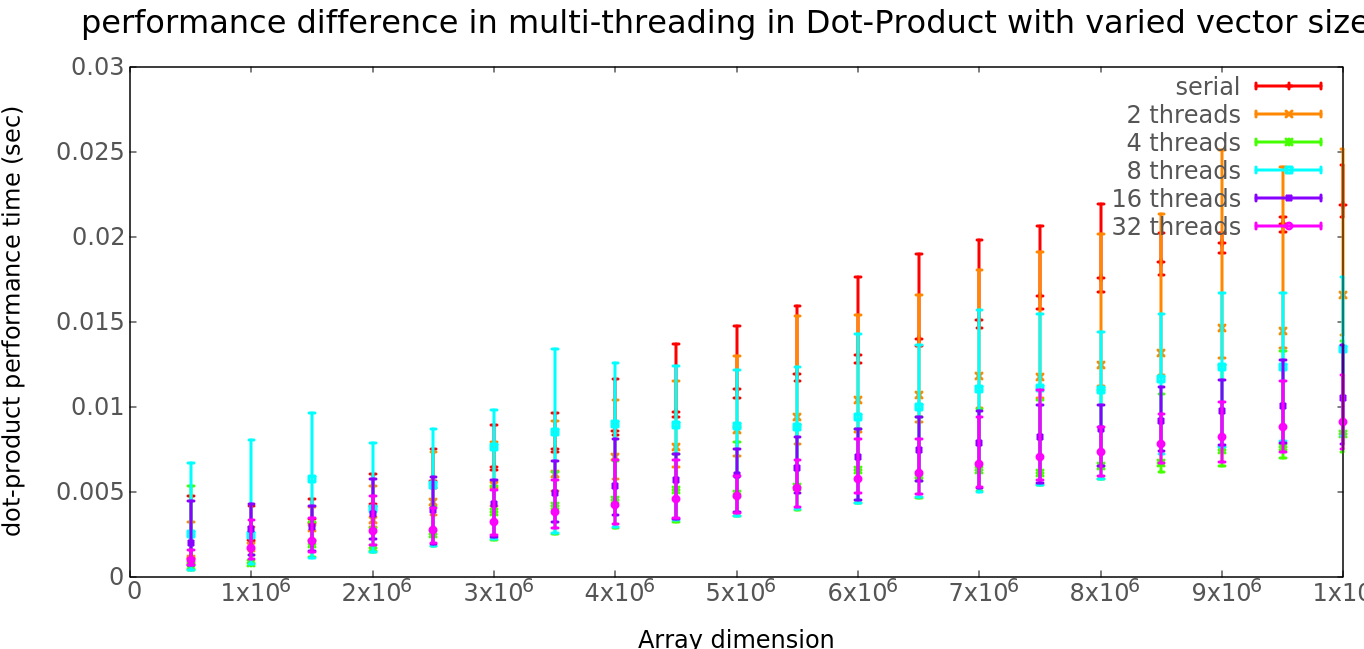
\includegraphics[width=1.00\textwidth]{graph2.png}
		\end{center}		
		\caption{scatter plot with error bars, using min, max and average}
	\end{figure}
	\textbf{1.2)} For small vector sizes, increasing the number of threads has unpredictable and erratic affects, as can be seen in figure 1, showing no improvement in the 1st sector of the graphs. \newline
	
	For larger vector sizes, the observed performance stabilizes with the threaded programs generally out-performing the serial one. The 4 threaded prgram performs the best while the 2 threaded program perfoms the worst after the serail version. \newline
	
	This observation makes some sense since it can be explained, in part, by the overheads incurred when attempting to parallelize code. One would expect parallelization to improve performance immediately, but would only be able to overcome the overheads and show a significant improvement with larger data-sets. 4 threaded program performs best because it seems to optimally take advanatge of resources (cores and such) while minimising overheads. \newline
	
	\textbf{1.3)} For smaller array sizes, no performance improvement was observed. For larger array sizes, a more positive stable linear relationship was observed, with 4 the threaded program having the lowest gradient
	
\end{document}
